\mode*

\begin{frame}
  \tableofcontents
\end{frame}

\section{Vem är jag?}

% Bakgrund: Att komma från Timrå och jobba på KTH, livets resa och genomförda 
% utbildningar.

\begin{frame}
  \begin{block}{Vem är jag?}
    \begin{description}
      \item[Namn] Daniel Bosk
      \item[Född] 1985 i Timrå
      \item[Jobb] Undervisar om programmering, datasäkerhet;\\
        forskar om datasäkerhet och didaktik på KTH.
    \end{description}
  \end{block}
\end{frame}

\section{Grundskola och gymnasium?}

\begin{frame}
  \begin{block}{Var gick jag i skola?}
    \begin{description}
      \alert<1-2>{\item[År 1--6] Laggarbergs skola, Timrå}
      \alert<3-4>{\item[År 7--9] Mariedalsskolan, Timrå}
      \alert<5-6>{\item[Gymnasiet] Naturvetenskapliga programmet, Timrå 
        gymnasium}\only<5-6>{\footnote{%
        Finns många studenter på KTH som gått andra program, t.ex.~Estetiska 
        programmet.
    }}
    \end{description}
  \end{block}

  \begin{figure}
    \only<1>{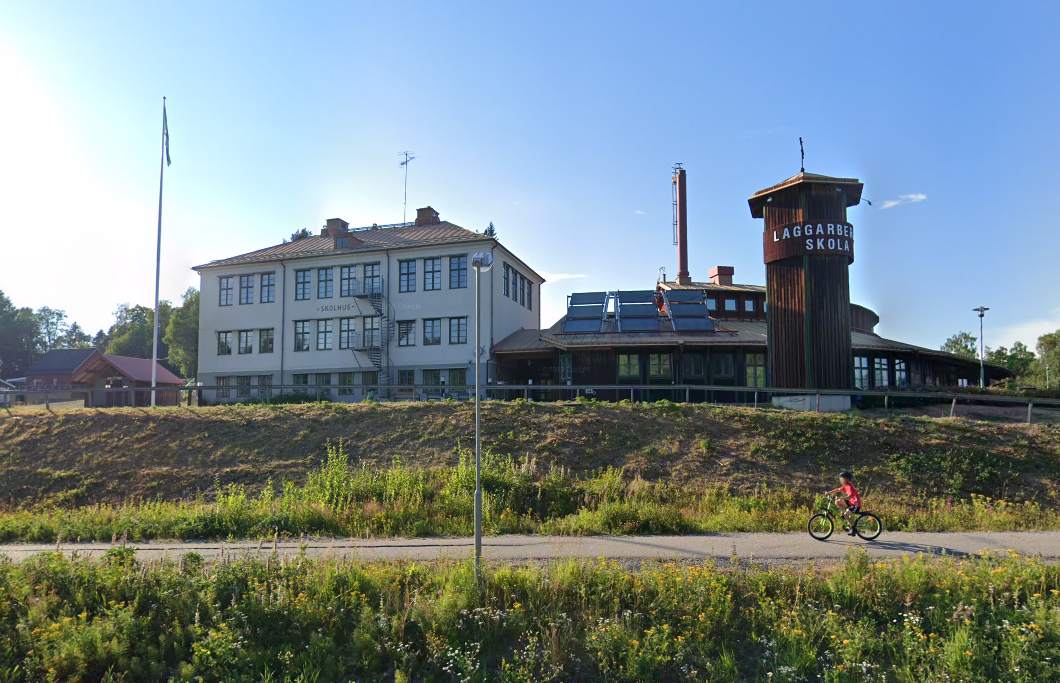
\includegraphics[height=0.5\textheight]{fig/laggarbergs-skola.png}}
    \only<2>{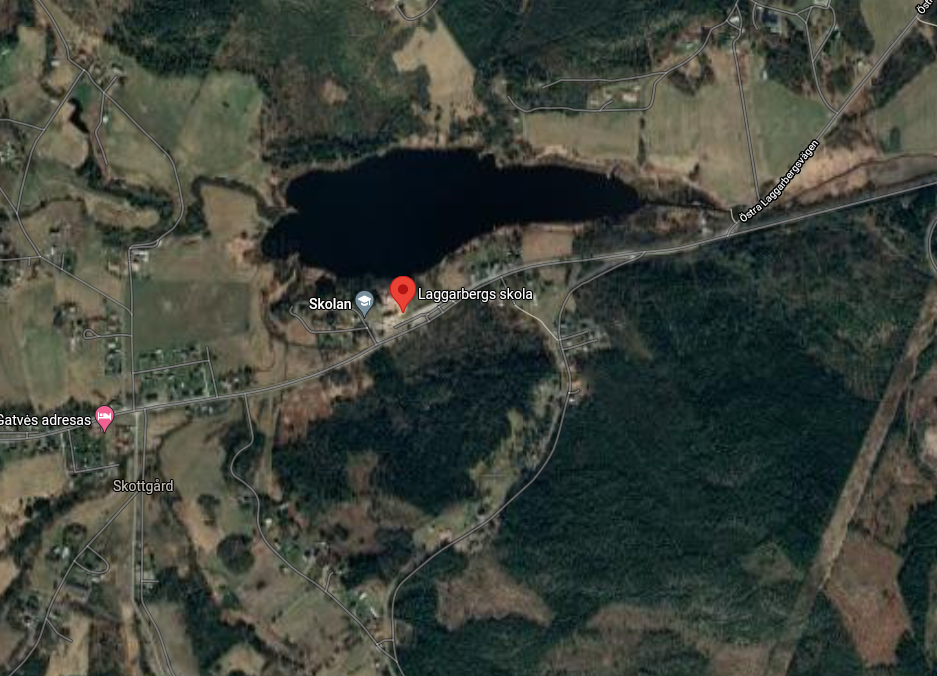
\includegraphics[height=0.5\textheight]{fig/laggarberg-close.png}}
    \only<3>{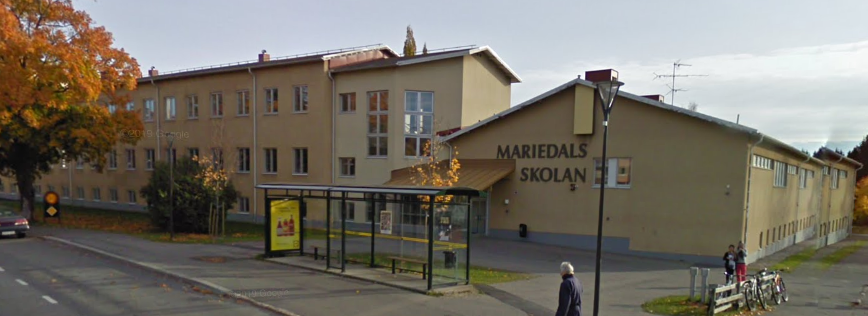
\includegraphics[height=0.5\textheight]{fig/mariedalsskolan.png}}
    \only<4>{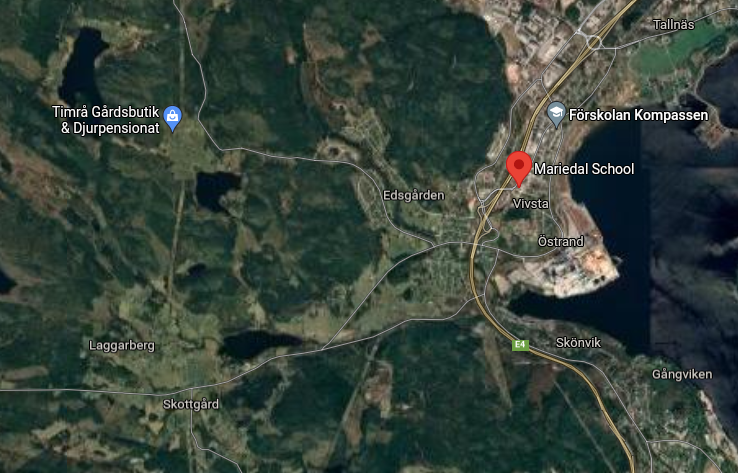
\includegraphics[height=0.5\textheight]{fig/mariedal-laggarberg.png}}
    \only<5>{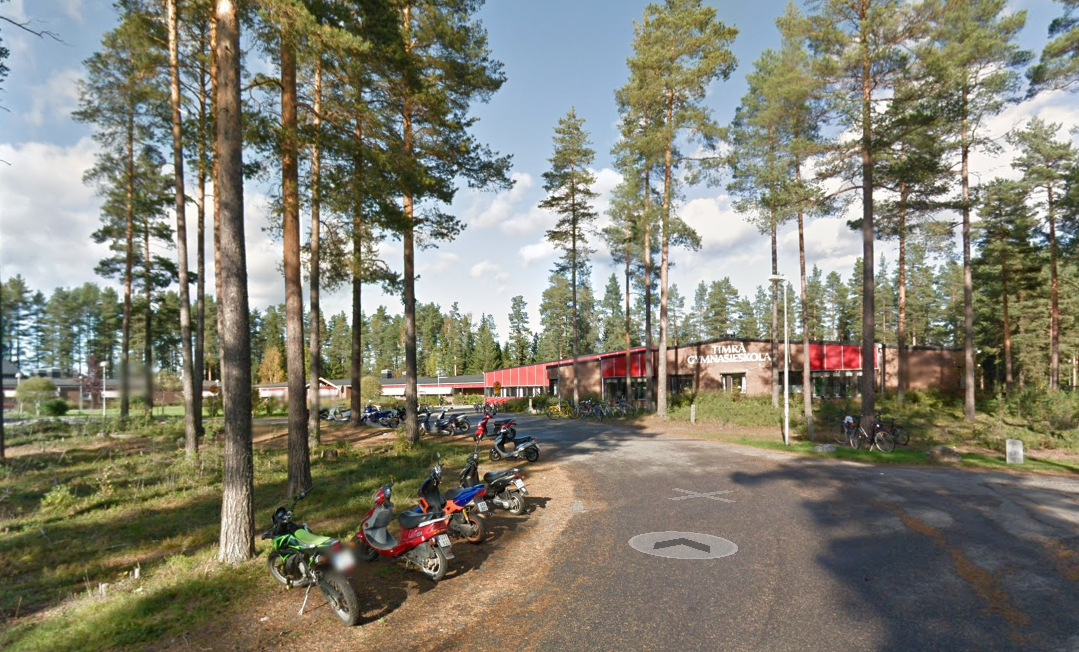
\includegraphics[height=0.5\textheight]{fig/tigy.png}}
    \only<6>{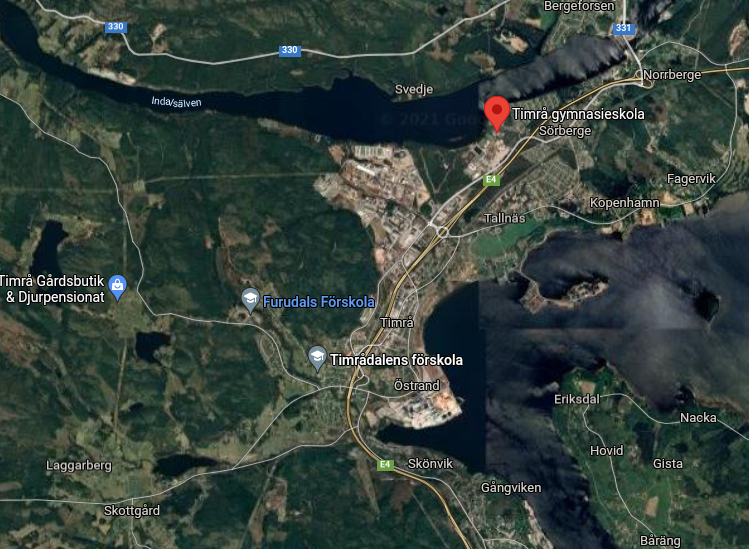
\includegraphics[height=0.5\textheight]{fig/tigy-map.png}}
    \only<1-2,4-6>{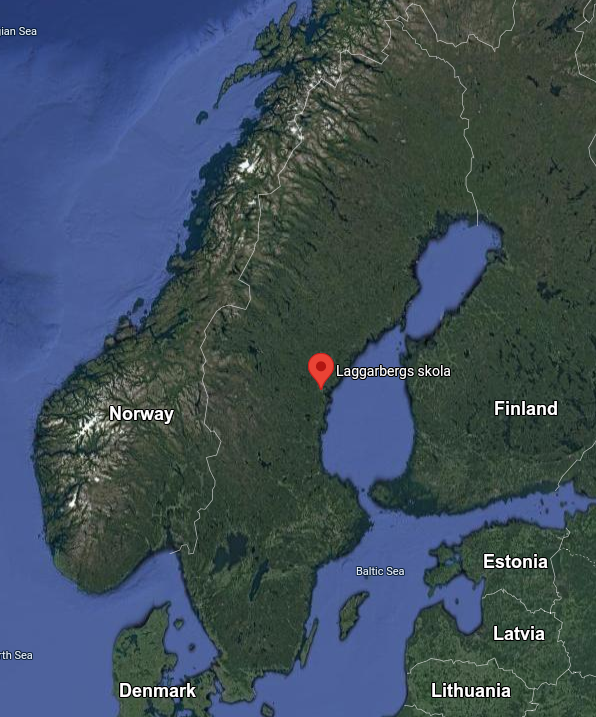
\includegraphics[height=0.5\textheight]{fig/laggarberg-sweden.png}}
  \end{figure}
\end{frame}

\section{Efter gymnasiet?}

\begin{frame}
  \begin{block}{Vad gjorde jag efter gymnasiet?}
    \begin{description}
      \only<1>{\alert<1>{\item[Uppehåll, 1 år] Värnpliktsutbildning, K4 
      Arvidsjaur.}}
      \alert<2>{\item[År 1]  Matematik, Mittuniversitetet}
      \alert<3-5>{\item[År 2--6] Civilingenjör- och lärarexamen i matematik och 
      datalogi, Kungliga Tekniska högskolan (KTH) och Stockholms universitet}
      \alert<4-5>{\item[Våren 2011] Resurslärare i matematik, Sörbergeskolan, 
      Timrå}
      \alert<6-7>{\item[Hösten 2011] Universitetsadjunkt i datateknik, 
      Mittuniversitetet, Sundsvall}
    \end{description}
  \end{block}

  \begin{onlyenv}<5>
    \begin{exampleblock}{Våren 2011}
      \begin{itemize}
        \item Gjorde examensarbetet för lärarutbildningen i matematik, 
          gymnasiet.
        \item Undervisade åk 7--9 i matematik.
        \item Undervisade åk 7--9 i teknik (programmering i Python).
      \end{itemize}
    \end{exampleblock}
  \end{onlyenv}

  \begin{onlyenv}<7>
    \begin{exampleblock}{Undervisning 2011--}
      \begin{itemize}
        \item Introduktion till datorteknik, Operativsystem, Programmering, 
          Människa--datorinteraktion, Nätverks- och webbsäkerhet
        \item Informationssäkerhet
      \end{itemize}
    \end{exampleblock}
  \end{onlyenv}

  \begin{figure}
    \only<2>{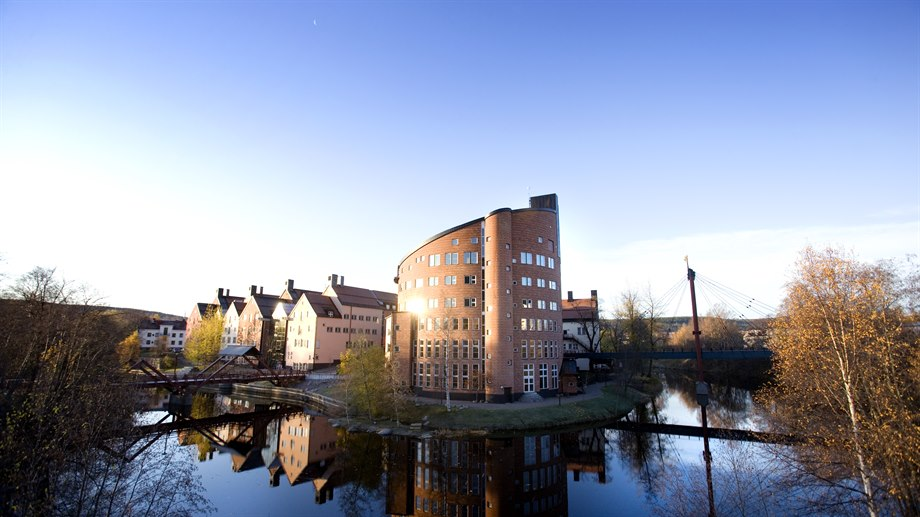
\includegraphics[height=0.35\textheight]{fig/miun.jpg}
    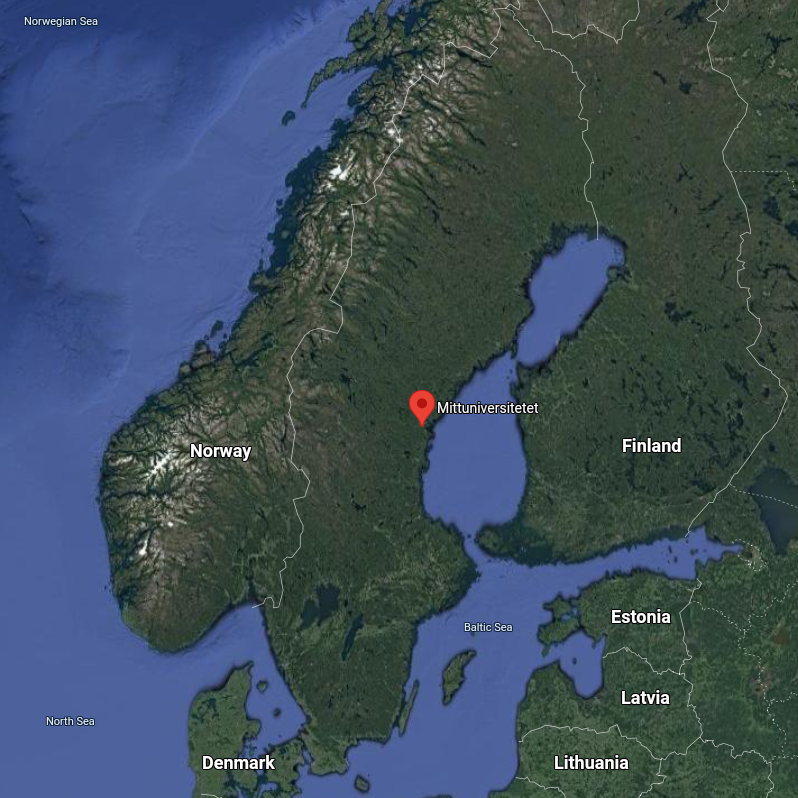
\includegraphics[height=0.35\textheight]{fig/miun-map.png}}
    \only<3>{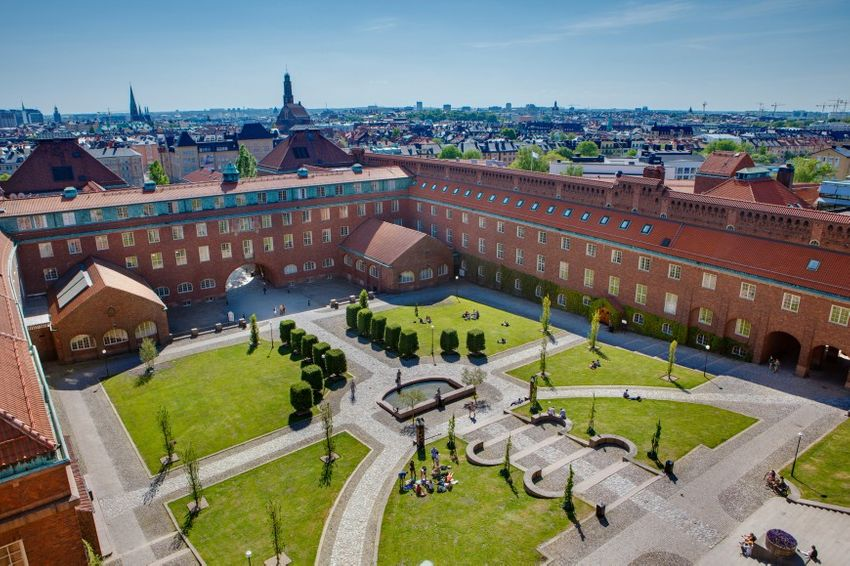
\includegraphics[height=0.35\textheight]{fig/kth.jpg}
    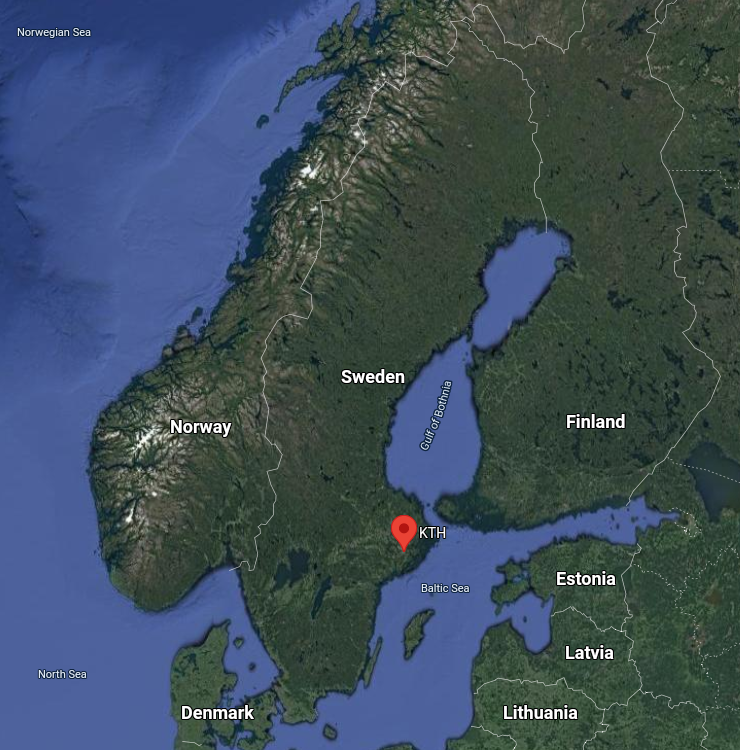
\includegraphics[height=0.35\textheight]{fig/kth-map.png}}
    \only<4>{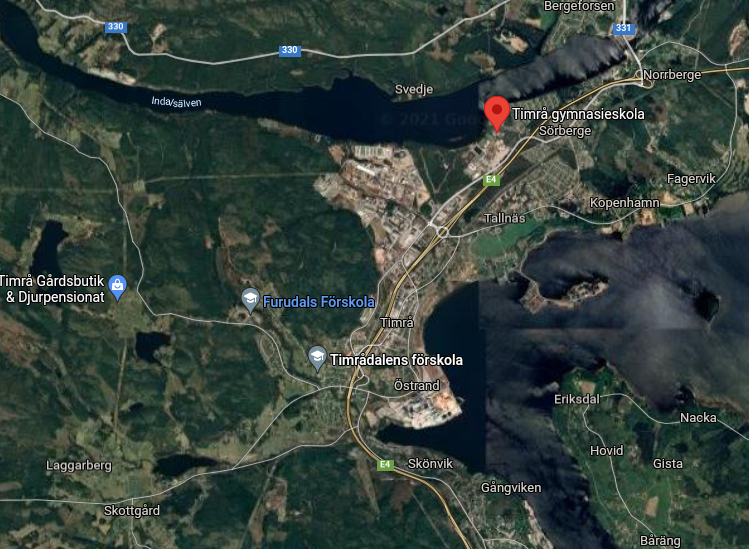
\includegraphics[height=0.35\textheight]{fig/tigy-map.png}
    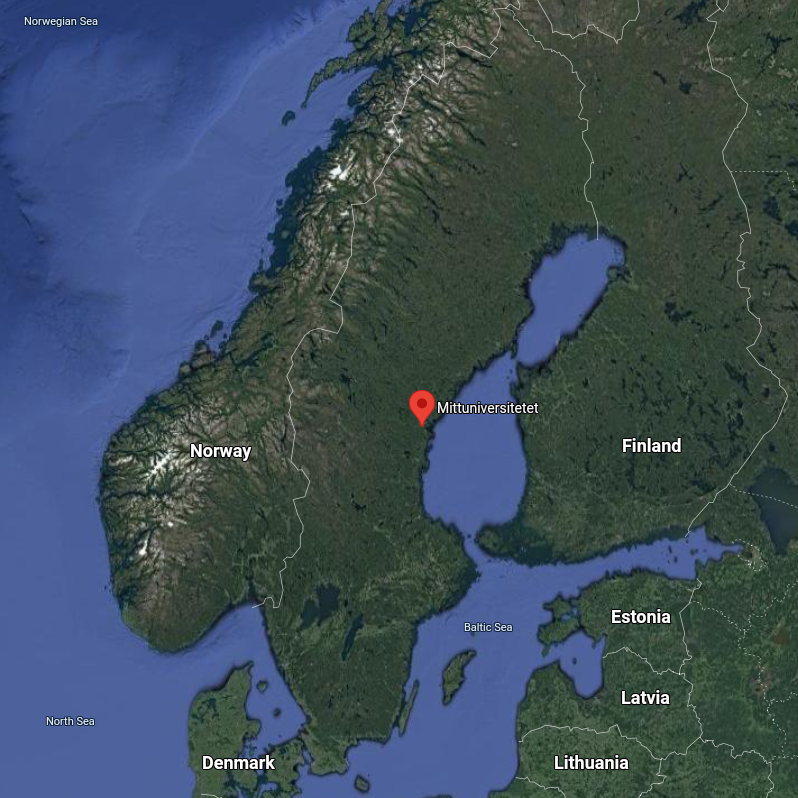
\includegraphics[height=0.35\textheight]{fig/miun-map.png}}
    \only<6>{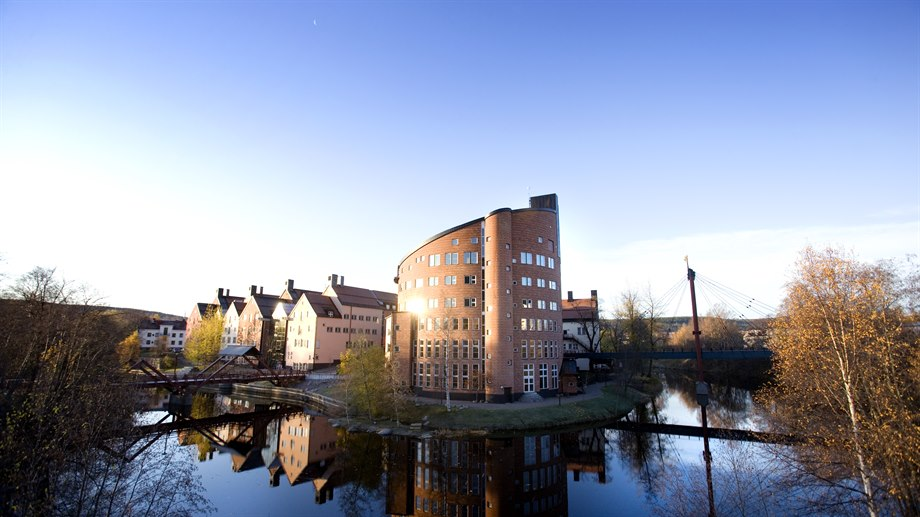
\includegraphics[height=0.35\textheight]{fig/miun.jpg}
    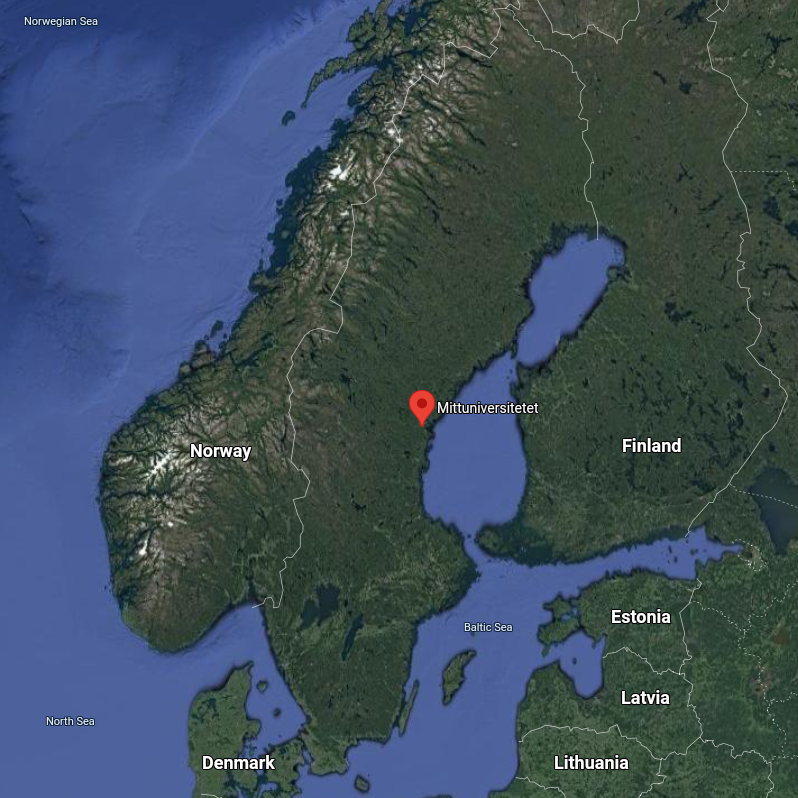
\includegraphics[height=0.35\textheight]{fig/miun-map.png}}
  \end{figure}
\end{frame}

\begin{frame}
  \begin{block}{Vad hände sedan?}
    \begin{description}
      \alert<1-2>{\item[Hösten 2011--2020] Universitetsadjunkt i datateknik, 
      Mittuniversitetet, Sundsvall}
      \alert<2-5>{\item[Hösten 2014--2020, år 7--11] Forskarutbildning 
      (doktorsexamen) i datalogi (tillämpad kryptografi), KTH}
      \alert<6>{\item[2020--] Universitetsadjunkt i datalogi, Kungliga Tekniska 
      högskolan, Stockholm}
    \end{description}
  \end{block}

  \begin{onlyenv}<1-2>
    \begin{exampleblock}{Undervisning \only<1>{2011--2014}\only<2>{2014--2020}}
      \begin{itemize}
        \uncover<1>{\item Introduktion till datorteknik, Operativsystem, 
        Programmering, Människa--datorinteraktion, Nätverks- och webbsäkerhet}
        \item Informationssäkerhet
      \end{itemize}
    \end{exampleblock}
  \end{onlyenv}
  \begin{onlyenv}<3>
    \begin{exampleblock}{Forskarstudier}
      \begin{itemize}
        \item Forskade om demokratifrämjande teknologier
        \item Anonymitet, autentisering, verifierbarhet
      \end{itemize}
    \end{exampleblock}
  \end{onlyenv}
  \begin{onlyenv}<6>
    \begin{exampleblock}{Just nu på KTH}
      \begin{itemize}
        \item Undervisar om programmering.
        \item Forskar och undervisar om säkerhet och tillämpad kryptografi.
        \item Forskar även om undervisning i programmering och säkerhet.
      \end{itemize}
    \end{exampleblock}
  \end{onlyenv}
  \begin{figure}
    \only<4>{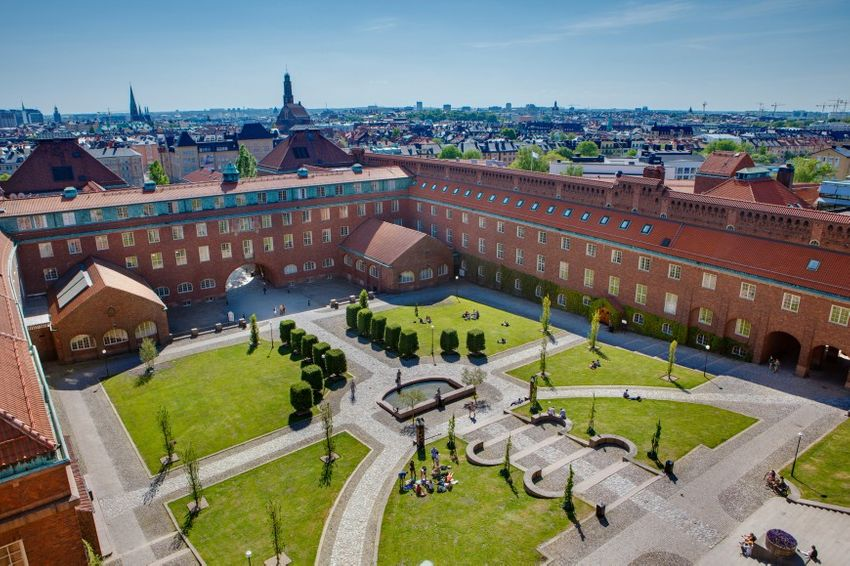
\includegraphics[height=0.35\textheight]{fig/kth.jpg}
    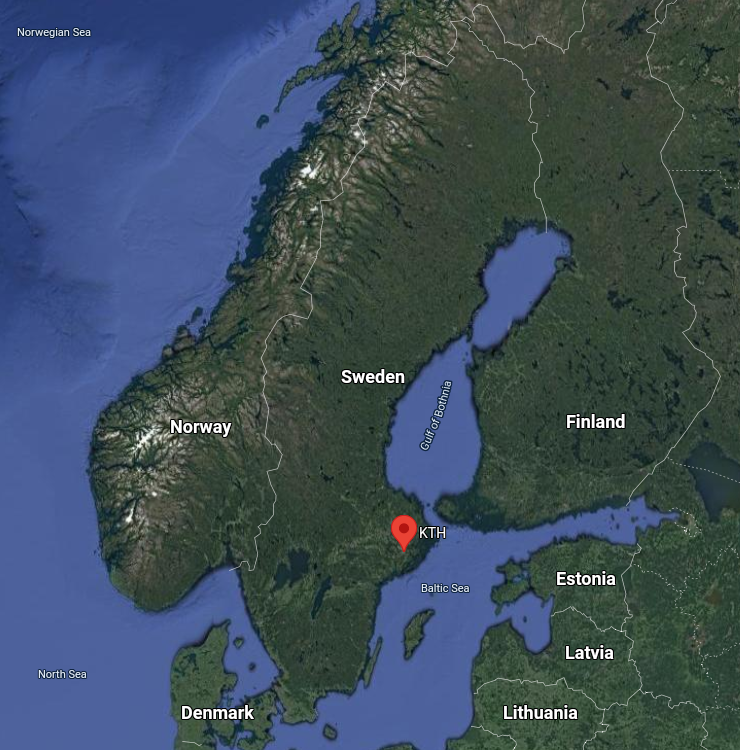
\includegraphics[height=0.35\textheight]{fig/kth-map.png}}
    \only<5>{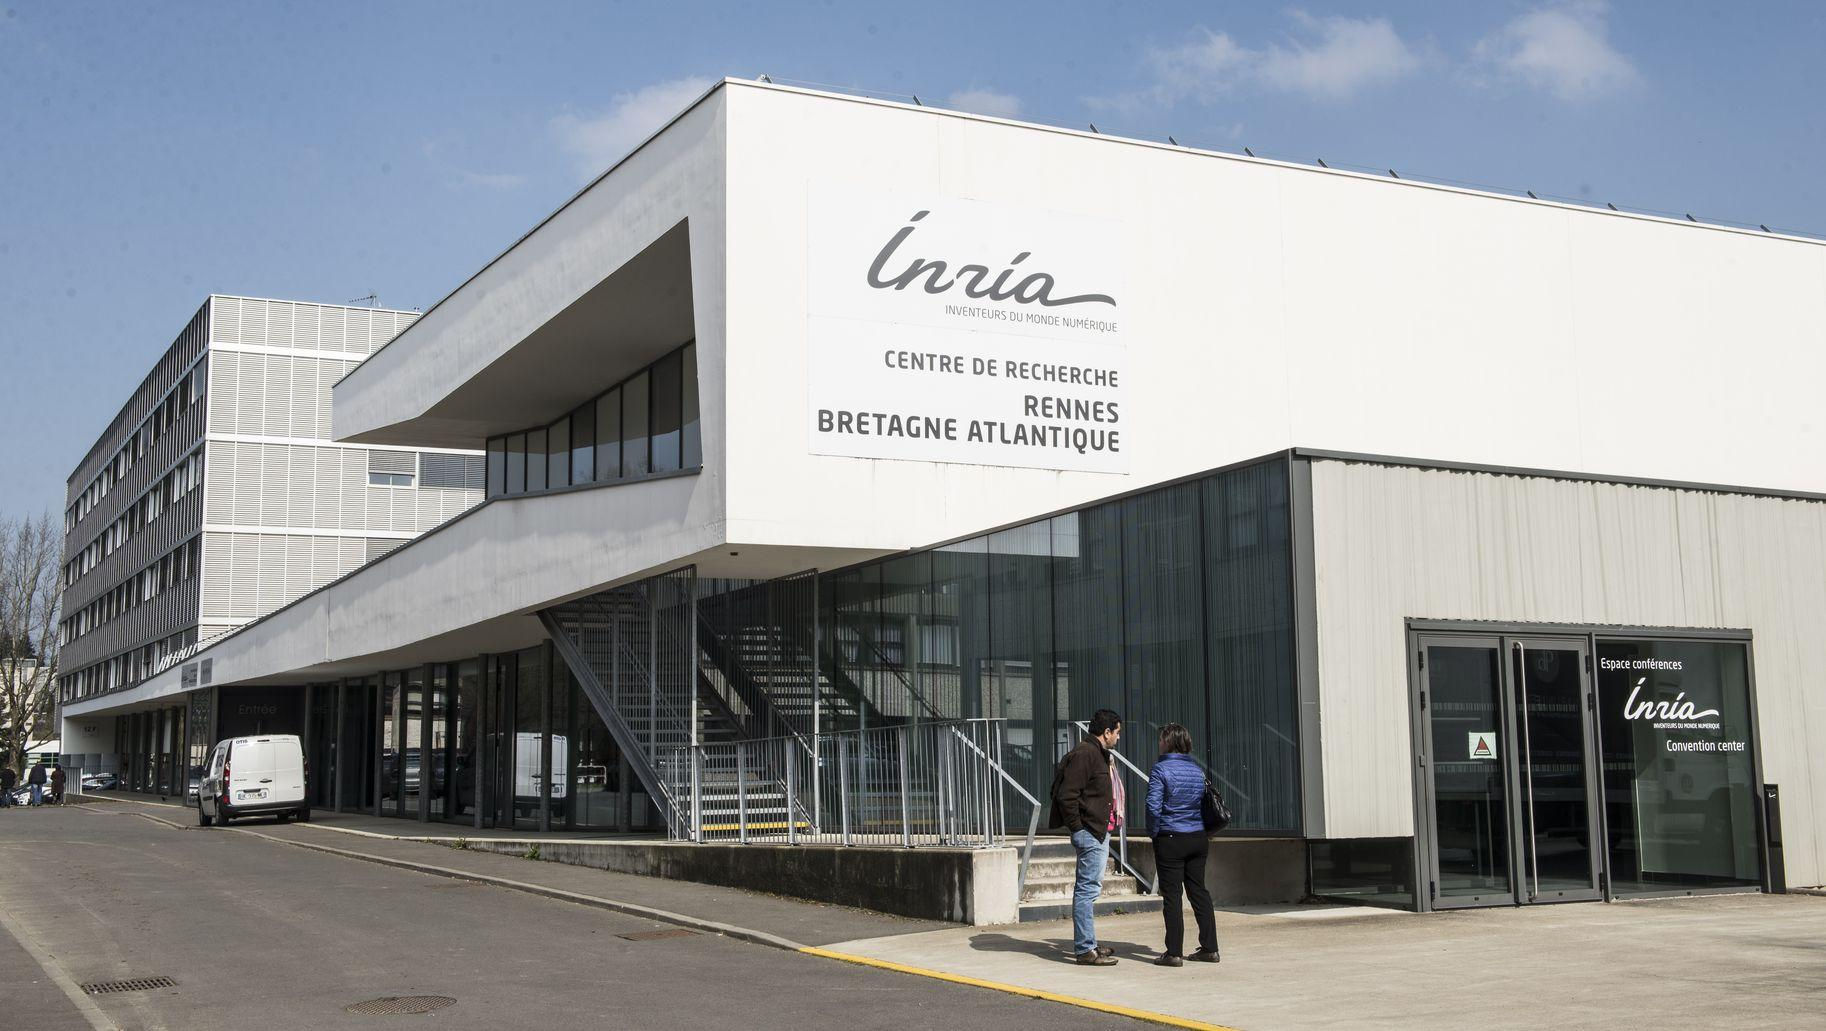
\includegraphics[height=0.4\textheight]{fig/inria-rennes.jpg}
    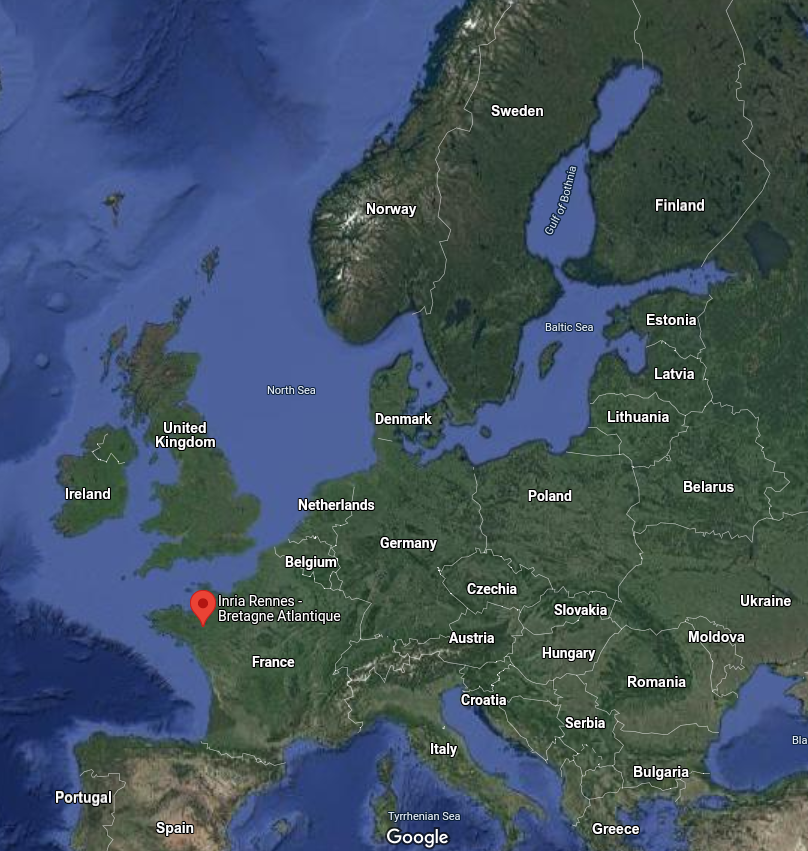
\includegraphics[height=0.4\textheight]{fig/inria-map.png}}
  \end{figure}
\end{frame}

